\documentclass[a4paper,10pt]{report}
\usepackage[utf8]{inputenc}
\usepackage{amsmath}
\usepackage{amssymb,amsfonts,textcomp}
\usepackage{array}
\usepackage{hhline}
\usepackage{hyperref}
\hypersetup{colorlinks=true, linkcolor=blue, citecolor=blue, filecolor=blue, urlcolor=blue, pdftitle=, pdfauthor=Gilles Vuidel, pdfsubject=, pdfkeywords=}
\usepackage{graphicx}
\usepackage[top=2.5cm,bottom=2.5cm,left=2.5cm,right=2.5cm,nohead]{geometry}
\usepackage{float}
\usepackage{parskip}
\usepackage{multirow}
\usepackage{caption}
\usepackage{fancyvrb}
\makeatletter
\newcommand\arraybslash{\let\\\@arraycr}
\makeatother
% centering figures
\makeatletter
\g@addto@macro\@floatboxreset\centering
\makeatother
\setlength\tabcolsep{1mm}
\renewcommand\arraystretch{1.3}

% saut après itemize
\let\EndItemize\enditemize
\def\enditemize{\EndItemize\medskip}


\begin{document}
\begin{titlepage}
	
	\centering
	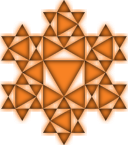
\includegraphics[scale=0.5]{img/logo.png}\\
	
	\bigskip
	\bigskip
	\bigskip	
	{\Huge
		\bfseries
		Fractalyse 3.0 (FracGIS)\\
		\bigskip
		User manual\\
	}
	\bigskip
	\bigskip
	\bigskip
	\bigskip
	\bigskip
	
	{\Large		
		Gilles Vuidel, Cécile Tannier and Pierre Frankhauser\\
		\bigskip
		2016-09-20\\
	}
	
\end{titlepage}

\parindent 0pt

\tableofcontents

\part{Generalities}

\chapter{Introduction}
\section{About Fractalyse 3.0}
Fractalyse is a software application for analysing 2D texture by fractal theory. 
The version 3 of Fractalyse has been completely rewritten in Java language, to improve data management with GIS (Geographical Information System) support, graphical user interface and performance with parallelism. It runs on any computer supporting Java Virtual Machine.
\section{Authors}
Fractalyse has been developed by Gilles Vuidel, Cécile Tannier and Pierre Frankhauser at ThéMA laboratory (University of Franche-Comté – CNRS). 
\section{Terms of use}
Fractalyse is distributed free-of-charge. Users must cite the following reference in their publications:
????
The source code is available and licensed in GPLv3.
\section{System requirements}
Fractalyse 3.0 runs on any computer supporting Java 1.7 or later (PC under Linux, Windows, Mac, etc.). However,
when dealing with very large datasets, the amount of RAM memory in the computer will limit the maximum image size that can be processed in a single run with Fractalyse. In addition, for some methods, processing power (CPU) will determine the speed of computing. For details, see section 8 below.
\section{Installing the software}
Fractalyse can be downloaded from http://www.fractalyse.org

Download and install Java 1.7+ from java.com. If you have a 64-bit operating system, it is best to install the 64-bit version of Java.
Download fractalyse-3.0.jar and launch it.

\chapter{Input data}
Fractalyse can read 2 types of data : vector and raster.
\section{Data type}
\subsection{Vector format}
Fractalyse support one vector format : Shapefile (.shp). This format is a vector GIS file format created by ESRI for its GIS ArcGIS.
It supports 3 type of geometry : point, line and polygon.
Fractalyse support all these geometry types. 

\subsection{Raster format}
Fractalyse support 2 raster formats : TIFF and Ascii Grid.

Ascii grid is a text format. The image is written as a matrix preceded by a header of 5 lines :
\begin{Verbatim}
	ncols	5
	nrows	5
	xllcorner	0
	yllcorner	0
	cellsize	1
	1 0 0 0 1
	0 1 0 1 0
	0 0 1 0 0
	0 1 0 1 0
	1 0 0 0 1
\end{Verbatim}

TIFF is a binary format commonly used for raster image. It can contains an extension named GeoTIFF, which added spatial references to the image. Fractalyse can load TIFF image with or without GeoTIFF extension. Fractalyse does not support RGB color image. You must convert your image in grayscale mode before using Fractalyse.

\chapter{Fractal methods}
This chapter explains the principles of the different fractal methods implemented in Fractalyse. 
\section{Unifractal dimension}
Fractalyse implements 3 methods to estimate the fractal dimension :
\begin{itemize}
	\item box counting
	\item dilation
	\item correlation
\end{itemize}

\subsection{Principles}
Fractalyse implements different methods (box counting, dilation, correlation...) to measure fractal dimension which corresponds to different dimensions (Hausdorff, Minkowski, Correlation...). The process of the measure is split in two part :
\begin{itemize}
	\item the counting method
	\item the estimation module.
\end{itemize}

\subsubsection{The counting method}

Counting method goes step by step following an iteration principle. At each iteration step, the method involved counting the number of black pixels contained in a counting window. From one step to the next, the size of the counting window is enlarged. By doing that, we artificially change the level of analysis of the image. So, for each method we have two elements varying according to the counting step (iteration step) (i):
\begin{itemize}
	\item the number of counted elements ($N$)
	\item the size of either the counting window or the reference element ($\epsilon$).
\end{itemize}
	
Then, we obtain a series of points that can be represented on a Cartesian graph. The Y-axis corresponds to the number of counted elements ($N$) and the X-axis corresponds to the size of the counting window or to the size of the reference element $\epsilon$, with $\epsilon$ increasing from step to step.

\subsubsection{The estimation module}

Mathematically, the series of points is a curve (named the empirical curve). The next stage is to fit this empirical curve with another one, the estimated curve. If the empirical curve follows a fractal law, the estimated curve has the form of a power law (parabolic or hyperbolic), and D represents the fractal dimension.
$$N = \epsilon^D or N = \epsilon^-D$$
In most cases, the empirical curve is transformed on a log-log plot. The estimation of the fractal dimension becomes a linear regression.
$$\log N = \log \epsilon^D = D \log \epsilon$$

\subsection{Box counting}
This is the most used method to estimate fractal dimension. The image is covered by a quadratical grid and the grid resolution $\epsilon$ is then varied. Following the logic described earlier, for each value $\epsilon$, the number of squares $N(\epsilon)$ containing any occupied point is counted. 

\subsection{Dilation}
This method is based on the algorithm introduced by Minkowski and Bouligand to establish the dimension of an object using the measure theory approach. In this analysis each occupied point is surrounded by a square (or a circle) of size $\epsilon$, the surface of which is considered to be completely occupied. The size of these squares is then gradually enlarged, and we measure the total surface $A(\epsilon)$ covered at each stage. As the squares are enlarged, any details smaller than $\epsilon$ are overlooked and we gradually obtain an approximation of the original form. Because more and more squares overlap, the total occupied surface for a particular value $\epsilon$ is less than what it would be if the same number of occupied points that make up the original form were surrounded individually. By dividing this total surface by the surface of a test square ($\epsilon^2$) or circle ($\pi\frac{\epsilon}{2}^2$), we get an approximation of the number of elements $N(\epsilon)$ necessary to cover the whole.

\subsection{Correlation}
Each point of the image is surrounded with a small squared window. The number of occupied points inside each window is enumerated. This allows the mean number of points per window of that given size to be calculated. The same operation is applied for windows of increasing sizes. The X-axis of the graph represents the size of the side of the counting window $\epsilon = (2i+1)$. The Y-axis represents the mean number of counted points per window. (Because the theory underlying the correlation analysis considers the simultaneous presence of two points at a certain distance, i.e. the mean distance between a pair of built-up pixels, the correlation dimension is a second order fractal dimension. In a multi-fractal theoretical framework, this correlation dimension should be extended to a series of three, four or more points). In principle it is possible to choose any shape for the window, such as circle, hexagon, etc. However, since pixels are square-like, the choice of a square helps to avoid rounding errors.

\section{Local dimension}
\subsection{Radial}

\section{Multifracal}
\subsection{Dimension spectrum}
\subsection{Box counting}
\subsection{Wavelets}


\part{Graphical interface}

\chapter{Data}
Fractalyse can process 2 types of 2D data : vector and raster.
\section{Loading data : File menu}
\subsection{Load vector data}
Shapefile format is a vector GIS file format created by ESRI for its GIS ArcGIS.
This format supports 3 type of geometry : point, line and polygon.
Fractalyse support all these geometry types. 

When the shapefile is loaded with the menu "Load vector data", a new layer is created and displayed.

\subsection{Load raster data}
Fractalyse support 2 raster formats : TIFF and Ascii Grid.

When the image file is loaded with the menu "Load raster data", a new layer is created and the image is displayed. If the image contains only 0 and 1 value, Fractalyse set the layer as binary layer and set white color for 0 and black color for 1. Otherwise, it sets a gray scale color ramp for the image. Color image (RGB) are not supported.


\section{Data manipulation : Tools menu}
For some analyses the vector data type is not supported (for example correlation for lineal or polygonal geometry) and for raster data type, most analyses need binary image. Fractalyse contains some functions in Tools menu to convert vector to raster data (Rasterize menu) and to convert grayscale raster to binary (Binarize menu).

\subsection{Rasterize menu : convert vector to raster}
\begin{figure}[H]
	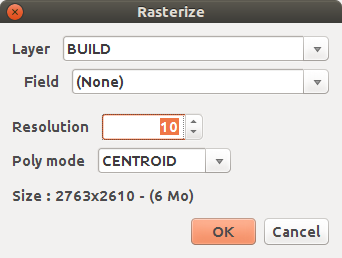
\includegraphics[scale=0.5]{img/rasterize-en.png}
\end{figure}

\subsection{Binarize menu : convert grayscale raster to black and white raster}
\begin{figure}[H]
	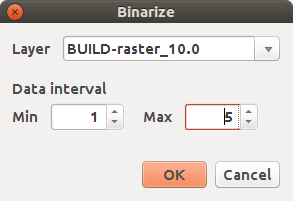
\includegraphics[scale=0.5]{img/binarize-en.png}
\end{figure}

\subsection{Negative menu : inverse binary raster}
Binary raster layer (ie. black and white) can be inversed by right clicking on the layer and select Negative menu item. Black pixels become white pixels and whites become blacks.

\subsection{Selection menu}

\chapter{Fractal analysis}
\section{Vector menu}
\subsection{Box counting}
\subsection{Dilation}
\subsection{Radial}
\subsection{Multifractal}
\subsection{Batch}

\section{Raster menu}
\subsection{Box counting}
\subsection{Dilation}
\subsection{Correlation}
\subsection{Radial}
\subsection{Multiradial}
\subsection{Multifractal}

\section{Network menu}
\subsection{Radial}
\subsection{Desserte}
\subsection{Backbone}

\chapter{Estimation module}
\section{Unifractal}
\section{Multifractal}

\chapter{Miscellaneous}
\section{Preferences menu}
\subsection{Memory}

\subsection{Processors}

\section{Log window}



\part{Command line interface}

\chapter{Prerequisite}

Fractalyse can be used in command line interface (CLI).
It is useful for executing Fractalyse on a distant computer without a graphical interface, or batching some processes that are not available in the graphical user interface (GUI).

\section{Launch Fractalyse in CLI mode}
First you have to open a terminal window.
Then, go to the directory of the Fractalyse program with \textit{cd} command.
Finally, type the following command to display the Fractalyse help screen :
\begin{Verbatim}
java -jar fractalyse-3.0.jar --help
\end{Verbatim}
Result
\begin{Verbatim}
Usage :
java -jar fractalyse.jar [-proc n]
...
...
\end{Verbatim}
You're ready to use Fractalyse in CLI mode !

\section{Syntax}
\subsection{Definition}
Commands always start with a double dash (\verb|--|).\\
A global option starts with only one dash (\verb|-|).\\
A parameter does not have a dash.\\
\subsection{Character separator}
Blank spaces are used to separate commands and parameters. You cannot have a name containing blank spaces.\\

\subsection{Optional parameter}
Parameters enclosed in brackets are optional. 
Therefore, parameters not in brackets are mandatory.


\subsection{Command execution}
Fractalyse can execute only one command.

\begin{Verbatim}
java -jar fractalyse-3.0.jar ...
\end{Verbatim}




\chapter{Command reference}
\section{General command}
\subsection{--help : display help}
Command :
\begin{Verbatim}
	java -jar fractalyse-3.0.jar --help
\end{Verbatim}

Result :
\begin{Verbatim}
Usage :
java -jar fractalyse.jar [-mpi | -proc n] COMMAND
COMMAND:
	--rasterize [neg] res=val file_1.shp [... file_n.shp]
	--binarize min=val max=val file_1.tif [... file_n.tif]
	--boxcounting SAMPLING [gliding=val] [estim=log|direct] file_1.shp [... file_n.shp]
	--rboxcounting SAMPLING [estim=log|direct] file_1.tif [... file_n.tif]
	--dilation SAMPLING [estim=log|direct] file_1.shp [... file_n.shp]
	--rdilation SAMPLING [estim=log|direct] file_1.tif [... file_n.tif]
	--correlation SAMPLING [estim=log|direct] file_1.tif [... file_n.tif]
SAMPLING: 
	[coef=val] [min=val] [max=val] [seq=arith|geom]
\end{Verbatim}

\section{Data manipulation commands}
\subsection{--rasterize : convert vector to raster}
\begin{Verbatim}[commandchars=\\\{\}]
--rasterize [neg] res=\textit{val} \textit{file_1.shp} [... \textit{file_n.shp}]
\end{Verbatim}

\subsection{--binarize : convert grayscale raster to binary}
\begin{Verbatim}[commandchars=\\\{\}]
--binarize min=\textit{val} max=\textit{val} \textit{file_1.tif} [... \textit{file_n.tif}]
\end{Verbatim}

\section{Fractal analysis commands}

\subsection{--boxcounting : box counting on vector data}
\begin{Verbatim}[commandchars=\\\{\}]
--boxcounting SAMPLING [gliding=\textit{val}] [estim=log|direct] \textit{file_1.shp} [... \textit{file_n.shp}]
\end{Verbatim}

\subsection{--rboxcounting : box counting on raster data}
\begin{Verbatim}[commandchars=\\\{\}]
--rboxcounting SAMPLING [estim=log|direct] \textit{file_1.tif} [... \textit{file_n.tif}]
\end{Verbatim}

\subsection{--dilation : dilation on vector data}
\begin{Verbatim}[commandchars=\\\{\}]
--dilation SAMPLING [estim=log|direct] \textit{file_1.shp} [... \textit{file_n.shp}]
\end{Verbatim}

\subsection{--rdilation : dilation on raster data}
\begin{Verbatim}[commandchars=\\\{\}]
--rdilation SAMPLING [estim=log|direct] \textit{file_1.tif} [... \textit{file_n.tif}]
\end{Verbatim}

\subsection{--correlation : correlation on raster data}
\begin{Verbatim}[commandchars=\\\{\}]
--correlation SAMPLING [estim=log|direct] \textit{file_1.tif} [... \textit{file_n.tif}]
\end{Verbatim}

\subsection{Sampling}
\begin{Verbatim}[commandchars=\\\{\}]
[coef=\textit{val}] [min=\textit{val}] [max=\textit{val}] [seq=arith|geom]
\end{Verbatim}

\section{Options}

\subsection{-proc}
Defines the number of processors (or cores) used by Fractalyse.
By default, CLI mode uses the value defined in the preferences window.
See the parallelism section for more details.

\subsection{-mpi}

\chapter{Command examples}
The following command will binarize all tif images contained in the current directory. For each .tif file, it will create a new one where each pixel having a value between 1 and 10 will be set to 1 and others to 0. Each new file will have a name with the suffix: \verb|_bin1-10.tif|.
\begin{Verbatim}
	java -jar fractalyse-3.0.jar --binarize min=1 max=10 *.tif
\end{Verbatim}

The following command will calculate the fractal dimension with box counting method for each images previously binarized.
\begin{Verbatim}
	java -jar fractalyse-3.0.jar --rboxcounting coef=1.5 *_bin*.tif
\end{Verbatim}

\chapter{Performance tuning}
\section{Parallelism to speed up execution}
\subsection{One computer : threads}
If your computer has more than one core (most of them), you can take advantage of parallelism. 
Most Fractalyse commands are parallelized. You can speed up command execution by defining the number
of cores (or processors) used by Fractalyse with the option \textit{-proc} after the project command :
\begin{Verbatim}
	java -jar fractalyse-3.0.jar -proc 8 ...
\end{Verbatim}
By default, CLI mode uses the number of processors defined in the preferences window of the GUI.
\subsection{Computer cluster : mpi}
Fractalyse can be run on computer clusters wich support Java for OpenMPI.
\begin{Verbatim}
	mpirun java -jar fractalyse-3.0.jar -mpi  ...
\end{Verbatim}
Only some commands can be used in mpi environments : 
\section{Memory management}
In CLI mode, the memory configuration defined in the preferences window cannot be used.
By default, the amount of memory available for Fractalyse is system dependent. It can vary from 128 Mb to several Gb.
In most cases, Fractalyse will run normally. But if you have a large image, some commands would be slow or even crash due to memory limitation.
If Fractalyse execution terminates with OutOfMemoryError, GC overhead or Java Heap space, you need to increase memory allocated to Fractalyse.

To define manually the maximum amount of memory allocated to Fractalyse, use Java option -Xmx :
\begin{Verbatim}
	java -Xmx2g -jar fractalyse-3.0.jar ... # 2Gb allocated
	java -Xmx1500m -jar fractalyse-3.0.jar ... # 1500 Mb -> 1.5Gb allocated
\end{Verbatim}
If you cannot allocate more than 1Gb or 1.5G and your computer has more memory available, you have probably a 32-bit version of Java, which is limited to less than 2Gb of memory.
Check your Java version :
\begin{Verbatim}
	java -version
\end{Verbatim}
If it is a 32-bit version, install a 64-bit Java version to handle all your computer memory.

\end{document}          
